\chapter{Introduction}
This research was inspired by learning about the power and capabilities of applying usage data collected by mobile apps in extremely popular real-world mobile apps in the early days of mobile apps (before Android, iOS and other modern mobile platforms were released). 
Several years later, when consulting with another company with over ten million active users I discovered they had included two analytics tools in their apps where there were numerous discrepancies in the data collected, the ways the counted and the resulting reports, yet they were both considered necessary. The engineers then added a third analytics library in the hope it would correlate with one or other of the existing libraries - it didn't, instead it had distinct characteristics and counts. And yet the developers were able to discover how their apps were used in incredible detail and by applying what they learned their apps became increasingly popular and financially successful.

These experiences led me to starting my PhD in order to research the potential of mobile analytics, and to understand some of their flaws and the effects of those flaws. During my research there have been incredible changes in the mobile landscape (for instance major manufacturers, operating systems, etc. have appeared, mushroomed, and disappeared). Similarly many test automation tools and frameworks have been and gone. Meanwhile, apps and app stores have spread beyond smartphones and tablets to desktop operating systems, cloud-based product offerings such as Salesforce, etc. Google's Android platform includes platform-level data collection, reporting and analytics intended to help developers learn about ways they can improve their apps. Meanwhile regulation has started to emphasise and highlight some of the many risks and concerns with gathering data wantonly. 

Despite all these changes, and my limited inroads into a subset of the entire landscape, the research seems to indicate the potential of applying usage analytics to improve both the product (the software) and the process (how the software is developed and tested). The research also identified flaws within analytics tools and also between analytics tools. Both the potential and the flaws appear worth sharing with researchers and with practitioners to help them chose and use analytics wisely.

\section{The Research}
Note: This section is aimed to replace the following section \href{my-contributions-in-this-thesis}{\emph{\nameref{my-contributions-in-this-thesis}}} which focuses on the author rather than the research.

Software app developers need to deliver software that can be used successfully by end users. To do so they need to be able to create software and distribute it so it is available to end users. End users need to be able to install and use that software. If the software is sufficiently usable, useful and behaves adequately they may continue to use it. Developers cannot assess \emph{a priori} whether their software will meet the needs and expectations of users, meet their needs, or the needs of their stakeholders. In short they do not know whether it will thrive.

One of the key considerations is whether the quality of their apps are adequate. There are many ways to assess quality of apps, including static analysis, in-person testing, and automated testing. Users may perform their own subjective assessments of quality and some of these users provide feedback in the form of ratings and reviews. 

Researchers have investigated these various sources of quality related information. My research concentrates on using sources of analytics related to usage of apps to help developers a) assess the quality of their current software, and b) improve the quality using the same analytics sources.

Conceptually there appear to be four broad layers of usage analytics, these are illustrated in Figure \ref{fig:four-layers-of-analytics-for-mobile-apps} and described next. They will be discussed in more detail in the  chapter titled~\href{chapter-applying-analytics-to-development-practices}{\emph{\nameref{chapter-applying-analytics-to-development-practices}}}. %MUST_DO decide whether layer and level are synonymous, and if not whether to use one term or the other. Anyway I'm aware I may be conflating both terms here and want to improve the precision of whichever term(s) I use. 

\begin{figure}[ht]
    \centering
    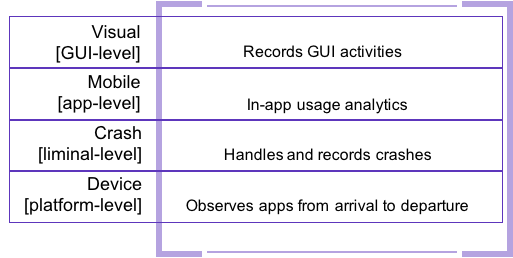
\includegraphics[width=12cm]{images/4-layers-of-analytics.png}
    \caption{Four Layers of Analytics for Mobile Apps}
    \label{fig:four-layers-of-analytics-for-mobile-apps}
\end{figure}

\begin{itemize}
    \item \textbf{Visual (GUI-level)} operates at the GUI level, or layer, of the app. It records aspects of the GUI activities such as touches, gestures, interactions with the screen, and data entry. Often it includes recording what is on the screen too. A common type of Visual analytics is \emph{heatmapping} software.
    \item \textbf{Mobile (app-level)} is incorporated as part of the app and records aspects of what the app is doing, in effect aspects of the usage of the app. Mobile Analytics is prevalent in Android apps and already used for various business purposes.
    \item \textbf{Crash (liminal-level)} is where specialised reporting can intercept crashes. Through the interception they can change the behaviour of the app, for instance to provide a better user-experience, log, and report the crash to the developers. \emph{Fatal crashes} are ones where the application quits. These can also be observed by the operating system; for mobile apps the operating system is an intrinsic part of the platform.
    \item \textbf{Device (platform-level)} Platform-level analytics can record apps from when they are installed until they are removed. This recording can include details such as when apps are in-use, crashes, freezes, and so on. Both of the dominant platforms (iOS and Google Android) allow users to decide whether their devices will share this data.
\end{itemize}

My research includes case studies and developer reports of examples of analytic tools that cover three of these four layers of analytics. The remaining layer, visual analytics, is described briefly with a few examples, visual analytics is seldom used in production mobile apps and therefore I decided to exclude these libraries from my core research. They may be an interesting topic for future research particularly given some of the potential benefits of visual analytics. % COULD_DO add notes on privacy issues and other complicating factors in this sort of research. 

\subsection{Research Problem}
Research into the use and efficacy of software usage analytics appears to be under-served, particularly in terms of being able to use the analytics to identify and potentially address quality flaws in apps in use. And in recent years, platform-wide analytics has been made available to all the developers of actively used Android apps in Google Play. Despite the ubiquity of these platform-level analytics there appeared to be no research into their efficacy, completeness, or accuracy.


\subsection{Research Contributions}
The research presents the results of several case studies in the use of analytics to improve the reliability of a variety of mobile apps.

TBC.

\subsection{Research Scope}


\subsection{Research Strategy}


\section{My contributions in this thesis}\label{my-contributions-in-this-thesis}
I have introduced the concept of using mobile analytics to help illuminate emergent behaviours of mobile apps and set mobile analytics into a broader context of other sources and reflections of perceived quality of mobile apps.

I have contributed the first studies into Platform Analytics as provided by Google Play Console, including pre-launch reports and Android Vitals, services intended to help developers identify quality issues with their Android apps in order to address these issues so they do not affect end-users. I have helped demonstrate their efficacy, despite various flaws I also discovered, identified and reported to Google. 

\begin{figure}[ht]
    \centering
    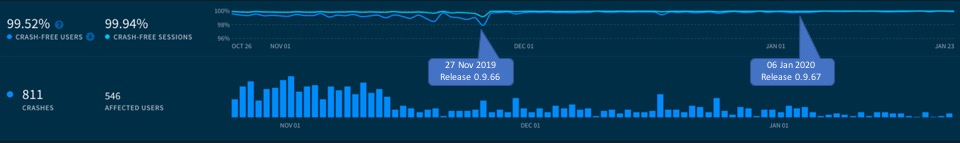
\includegraphics[width=\textwidth]{images/annotated_pocketcode_90_day_fabric_crashlytics_report.jpg}
    \caption{Pocket Code improvements in crash rate, in 90 days}
    %\Description{Pocket Code: When the project team investigated crashes they improved the reliability}
    \label{fig:pocketcode_improvements_in_crash_rate}
\end{figure}

Through my work with the key app created by the Catrobat project team we tamed their key Android app's crash rate that was previously precariously high\footnote{Nearly four times the maximum threshold recommended by Google in their Android Vitals service.}. The project team had not been able to address the crash rate despite applying many of the recognised and recommended software development practices over several years~\cite{adamsen2015systematic_catrobat, luhana2018streamlining, ali2019behavior_catrobat, ali2019using_catrobat, hirsch2019approach_catrobat, schranz2019contributors_catrobat, slany2014tinkering}. Owing to my involvement we were able to achieve this within 90 days and 2 releases through several small improvements to the codebase of the app, as Figure \ref{fig:pocketcode_improvements_in_crash_rate} shows.

\akb{I think you need to emphasise the role of analytics over your personal role above}

I also compare Crashlytics reports with the Platform Analytics and again identify both internal and cross-tool flaws and inconsistencies. Some of these have already been reported to Google in preparation for a full report to be submitted on completion of some ongoing research.

\begin{figure}[ht]
    \centering
    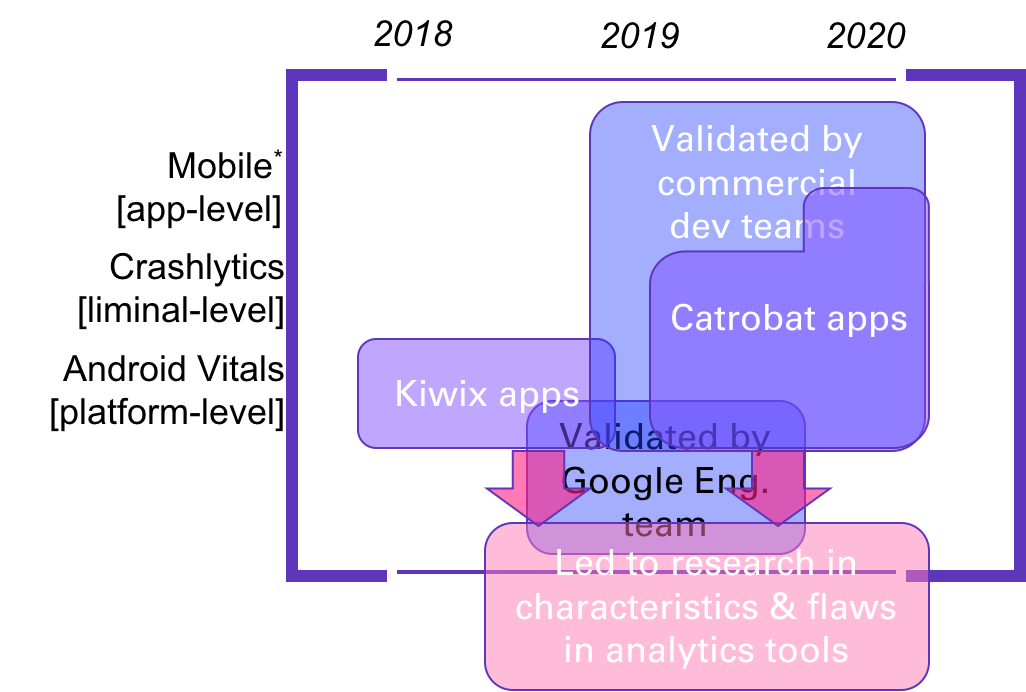
\includegraphics[width=10cm]{images/visual-connections-in-research.png}
    \caption{Visual Connections in my research}
    \label{fig:visual-connections-in-research}
\end{figure}

Figure \ref{fig:visual-connections-in-research}  aims to provide a visual overlay of the main practical elements of the research from 2018 to 2020. There are three main factors: 1) the type(s) of analytics used, 2) the development team and their apps, and 3) timescales.
\akb{Why is it important to understand the timeline here - what implication does it have for understanding the research problem?}

The research started with the Kiwix~\footnote{The Kiwix project enables people to use Wikipedia and other content offline~\url{https://www.kiwix.org/en/}} set of Android apps where the app with the highest crash rate, as reported by Google's Android Vitals, was used as the experiment to see if the crash rate could be improved. By design the Kiwix apps do not include any analytics or crash reporting to minimise the digital usage footprint of these apps as they may be used in areas of the world where Wikipedia is banned, \emph{etc.} where the users may be persecuted or even imprisoned. Nonetheless, as the apps were available through Google Play (amongst many sources) the development team received ongoing reports in Google Play Console including the Android Vitals reports on various `stability' metrics as defined and applied by Google. 

Google Play uses data collected automatically from users opted-in to provide usage and diagnostics data to Google. The data is collected at a per-device level, which means that one device could potentially report data from several user accounts, conversely for users who use multiple devices some may provide the data while others do not.

The Catrobat team was and is an extremely well researched and supported collection of mobile apps intended to help young people learn how to enjoy developing games visually. It was established by Professor Wolfgang Slany of the TU Graz university where both undergraduate and postgraduate students actively practice software skills on the codebase. My engagement started around June 2019 and we jointly decided to pick the thornier and most complex Android app - Pocket Code - as the subject for our collaboration and research as it had proved to have an intractable ongoing issue with the high reported crash rate and therefore a worthy challenge for the concepts proposed in my research. We had a reference app, called Pocket Paint, which had a lower crash rate. Note: Pocket Paint was and is incorporated into Pocket Code in addition to being a standalone app.

Pocket Code already incorporated one of the most popular crash analytics library called Crashlytics. At the time, it used an older, mature version of Crashlytics branded Fabric (a business first acquired by Twitter, then by Google). I have chosen to use the term \emph{liminal}~\footnote{\url{https://www.lexico.com/en/definition/liminal}} to indicate crash reporting is something that lives in the boundary layer between the app and the operating system, or platform. Either is able to observe application crashes, and for apps where both the app and the platform capture information about crashes the two data sources can be usefully cross-referenced and compared, as my research has done.

As Pocket Code was an Android app, available in Google Play, the team also received the reports provided by Google through Google Play. These two data sources provided an interesting and rich set of research challenges. 

Relatively recently, in February 2020, the Catrobat team had to migrate their Crashlytics reporting from the Fabric service, which Google was ceasing, to Firebase the replacement reporting service Google provided. In parallel with this migration of the reporting the project team agreed to incorporate mobile analytics into their Android and iOS apps. They decided to use Firebase Analytics for various reasons (to be covered later in my thesis), hence the extension of the apps into app-level analytics.

The two arrows in the figure indicate an area of unplanned research: 
%
I discovered various flaws in the developer-oriented reports Google provides to app developers who make their apps available in Google Play (approximately 2.9 million apps globally). This led initially to discussions with the relevant engineering teams for Google Play and Android Vitals at Google where they confirmed various flaws. They asked for ongoing updates on my findings and requested a report which I provided. Through our interactions and discussions I realised the merit of researching the characteristics and flaws in analytics tools, and particularly those provided by Google for Android developers. This research is ongoing and intended to continue post PhD given the importance and relevance of the topic.

In mid-2019 several commercial Android development teams learned of my research and offered to contribute their experiences and practices of using mobile analytics in their commercial apps. These apps include app-level analytics in addition to the development teams receiving the ongoing reports Google provides automatically. The contributions of these development teams helped provide additional weight to the value and relevance of using mobile analytics to identify flaws in mobile apps and evidence of the importance developers placed on addressing quality issues gleaned through these tools.

%\yy{The practical research}{Need to complete the sentences, what is liminal? Change Kiwix/Catrobat apps to "Kiwix/Catrobat teams"? }

I instigated and led the development of several opensource software utilities to help record and preserve reports and underlying failure data from Google Play Console and Android Vitals. We have successfully extended the capabilities of the utilities and further extensions are practical. Research benefits:
\begin{itemize}
    \item Evidence preserved for analysis:
    \item Data can now be compared and further assessed:
    \item Data and contents can be shared by developers of Android apps with other researchers - extending the body of knowledge about crashes (un-reliability) and ANRs (run-time unresponsiveness). \emph{bringing previously unknown data, practices and tools into the open so others can understand them, make more informed decisions, and perform further research.}
\end{itemize}

I made data available~\cite{harty_wama_dataset_examples} for further research based on data originally only made available to app developers. Larger volumes of data are available upon request.

The research has been presented at various conferences and workshops, including at NII Shonan in 2019 at meeting 152 on "Release Engineering for Mobile Applications"~\footnote{~\url{https://shonan.nii.ac.jp/seminars/152/}}. 

\section{Outline of this thesis}
Bugs are ubiquitous in software (even one of the most respected software engineers, Donald E. Knuth, recognises, publicly acknowledges, \emph{and pays for}~\cite{knuth_trutex, wikipedia__knuth_reward_checks_2020} bugs found in his creations. And self-aware developers expect there will be bugs in their software. \emph{``You are entitled to a reward of at least 0x$1.00 ($2.56) if you are the first person to report a bona-fide error not on those lists."} Donald E. Knuth~\cite{knuth_the_bank_of_san_serriffe}

Even top development teams are likely to learn of bugs they were not able to find, and cannot reproduce. For instance, Google's Android Auto Team have asked for help from end users to identify patterns that may help the team find and address a long-running and frustrating bug in Android Auto~\footnote{\url{https://support.google.com/androidauto/thread/2865341?msgid=44437416}}. As reported by \texttt{autoevolution} in May 2020:  
\emph{"As it turns out, the Android Auto team wasn’t able to reproduce the whole thing, so it’s now asking users to send additional reports with more information to help fix the problem."}~\footnote{~\url{https://www.autoevolution.com/news/google-wants-users-to-help-fix-widespread-android-auto-bug-143760.html}}.

Developers want and need to know how well their apps are performing from various perspectives such as: growth and adoption (\emph{``do we have more users and are they using the app [more] often?"}), users' ratings and reviews (\emph{``do they like our work?"} and in terms of quality (\emph{``does it perform well? is it fast and reliable?"}). 

\begin{figure}[ht]
    \centering
    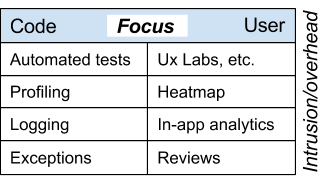
\includegraphics{images/ComparingTechniquesRHS.png}
    \caption{Comparing Techniques}
    \label{fig:comparing_techniques}
\end{figure}

There are various techniques that can be used to assess aspects of quality of mobile apps. Figure \ref{fig:comparing_techniques} provides a visual overview of eight techniques. Of these four are code-oriented and the remaining four more user- or usage- oriented. They are ordered in approximate rank of the overhead, effort, or intrusion involved of each technique. % MUST_DO continue and expand this argument. Discuss why exceptions were chosen as one of the core elements of my research and PhD thesis.

Google's Google Play app store provides developers with answers to all these niggling questions through a developer-oriented user interface called Google Play Console. 
In Google Play Console they provide various tools, reports and data all aimed at informing developers about how their apps are 'doing' and performing. Broadly, these include an overview page with one line of pre-selected data per app managed by the Google Play \textit{Developer Account}. Then, per app, Google provides an overview dashboard of graphs \emph{TODO add screenshot?}\yy{}{Yes, please, but needs a brief explanation too} which, in turn, link to more detailed reports and information which provide greater depth. Some graphs only appear when Google's algorithms decide they are relevant, these seem to be related to events and/or volumes of underlying data.

\subsection{Mobile app development lifecycle}
To provide some context for this section, Figure \ref{fig:ci-cd-development-and-feedback}~\footnote{Reproduced from \emph{``An empirical study of architecting for continuous delivery and deployment"}~\cite{shahin2019empirical_study_architecting_cd}}
illustrates a modern continuous software lifecycle including feedback. We can observe several distinct stages in the development and deployment of software and the feedback each stage can provide. %MUST_DO check the guidelines for reproducing and citing a figure as-is.

In contrast, Figure \ref{fig:google-play-app-development-and-feedback} illustrates a similar software lifecycle for Android apps released through Google Play together with the various forms of feedback~\footnote{Here we have excluded feedback from the app store, nonetheless it exists for many app stores.} 

Key differences between typical CI/CD lifecycles and the one for Google Play is the pre-launch testing and the app store providing both user feedback and a service called Android Vitals. The pre-launch reports are generated automatically by Google where the app store runs automated monkey testing on a farm of Android devices and various static analysis checks of releases deployed to any of the test channels. I will explain test channels later on. %MUST_DO actually add information on the test channels and how releases can be promoted to production releases in Google Play.

There are additional sources of \emph{analogue feedback} from people, including from alpha and beta testers and end users; and \emph{digital feedback} from Google tools and from usage data collected from the field. These terms are expanded in the following section~\href{analogue-and-digital-feedback}{\emph{\nameref{analogue-and-digital-feedback}}}.


\begin{figure}[ht]
    \centering
    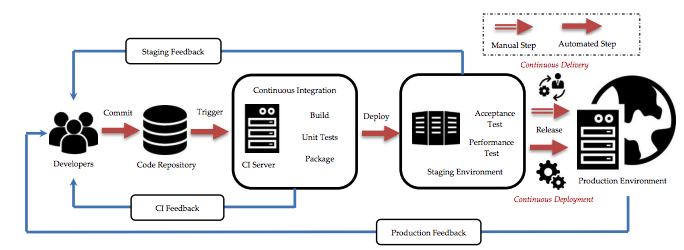
\includegraphics[width=13cm]{images/ci-cd-development-and-feedback.png}
    \caption{CI/CD development and feedback, reproduced from~\cite{shahin2019empirical_study_architecting_cd}}
    \label{fig:ci-cd-development-and-feedback}
\end{figure}

\begin{figure}
    \centering
    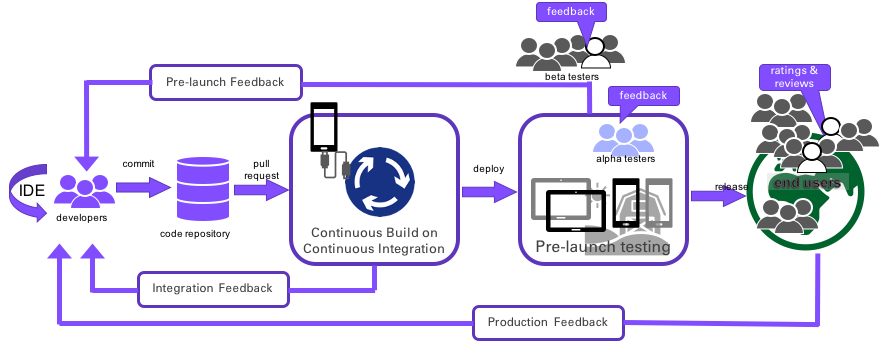
\includegraphics[width=13cm]{images/google-play-app-development.png}
    \caption{Google Play App Development and Feedback}
    \label{fig:google-play-app-development-and-feedback}
\end{figure}


\subsection{Mobile app usage lifecycle}
Mobile apps have a usage lifecycle, which starts when an app is chosen to be installed and ends with either abandonment or active removal of the app from a device. Figure~\ref{fig:mobile_app_usage_lifecycle}~\footnote{Based on a figure in~\cite{bohmer2011falling_asleep_with_angry_birds}} illustrates the possible stages of a mobile app's life on a user's device.

\begin{figure}[ht]
    \centering
    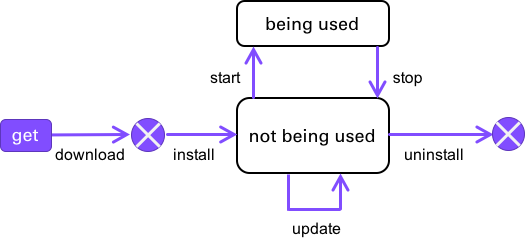
\includegraphics[width=12cm]{images/mobile_app_usage_lifecycle.png}
    \caption{Mobile App Usage Lifecycle}
    \label{fig:mobile_app_usage_lifecycle}
\end{figure}

Chapter TBD provides details of my understanding of how Google collects the underlying data (they do not document, explain or encourage research in how their system works, We return to their behaviour and the effects later in this introduction). And the chapter \href{chapter-software-we-developed-for-google-play-console}{\emph{\nameref{chapter-software-we-developed-for-google-play-console}}} describes software we developed to help collect data from Google Play Console in order to facilitate both research and to enable developers to collect and use data...

Crashes are often considered a concrete measure of poor performance of software and there has been extensive research in crashes for Android applications, in particular. I suspect there are various reasons for the focus on crashes as an oracle for testing software, crashes are unambiguous (even if the causes are not) and they are also binary so easy to determine whether software has, or has not, crashed. 

Google launched a service called Android Vitals as a new, intrinsic part of Google Play Console in 2016/17 \emph{TODO confirm the date and revise this sentence} where they popularised a measure called \emph{Stability} to assess the quality of Android apps. Their measure includes both crashes and when an application freezes or is unresponsive for at least 5 seconds from a user's perspective, a term Google call Application Not Responding (ANR).

\subsection{Analogue and Digital Feedback}~\label{analogue-and-digital-feedback}
Feedback can help developers to find and choose ways to improve their software. Various researchers have investigated way to understand and use feedback provided by end-users, for instance, in ratings and reviews users provide to the app store. For the purposes of my research I term feedback people provide as \emph{analogue feedback} as it has the richness and complexity of analogue signals, and also challenges of processing and comprehension.

In contrast, digital feedback originates from software and is generally deterministic~\footnote{~\url{https://en.wiktionary.org/wiki/deterministic}}. For the purposes of my research I consider digital feedback as that provided by running software where programmers added code to programs to collect data that provides feedback about software use and certain behaviours of that software. The addition of the code may be automated, in part, or wholly, for instance by another program or script. As an example, AppPulse Mobile claims they can add analytics automatically without developers writing a line of code~\footnote{~\url{https://www.microfocus.com/en-us/products/apppulse-mobile-app-apm-monitoring/overview}}.


% Mobile Developer's Guide to the fifth dimension
% available from https://www.dropbox.com/s/no70z2hiod6z7o8/Fifth_Dimension_v1.pdf?dl=0 (took 20 - 30 mins to track down)

\subsection{The Reaper Cometh}
AppBrain is a business that actively monitors and reports on Android Apps in the Google Play Store. The business was founded by two ex-Google engineers, as I am. They state Google is actively culling Android apps from the Google Play store and estimate approximately 16\% of apps are \emph{"low quality apps"} and \emph{"unlikely to be useful"}~\footnote{\url{https://www.appbrain.com/stats/number-of-android-apps}} % Percentage of low quality apps: 16%


\subsection{Validation of the concepts}
My practical research focuses on two sets of Android applications, those of the Kiwix and Catrobat project teams. According to data and reports Google provides the development teams their active user-bases are 362,595 for the Kiwix project across 18 published apps, and 148,966 for the Catrobat project across 6 published apps. %data obtained on 16th May 2020.
TODO map these apps to the buckets in the table from the 'beyond Google Play' paper.

While these apps include a useful variety of user populations (from 10's of users to 150K+ across many countries and tens of apps) they could be perceived as a \emph{drop in the ocean} of the millions of apps currently available in the Google Play app store. Also, both project teams are non commercial, and may have different working dynamics from commercial development projects and teams. As my research was inspired from my consulting work with businesses who rely on the success of their apps I chose to supplement these two projects by engaging with developers from several commercial development teams. These include: Moonpig, Moodspace, and LocalHalo. Each values and uses analytics data during their development process to assess post-launch issues with their apps. From time to time things go awry with the behaviours of one or more of their releases and analytics helps them to identify and respond to issues before they become pervasive. For the LocalHalo app, \emph{TODO add details}... For Moonpig \emph{TODO add details}...

\subsubsection{Validation by the Google Engineering Team}
In Spring 2019 I reported various flaws or potential anomalies in various reports Google Play Console provides to developers to the then Product Manager for Android Vitals, Mr Fergus Hurley. As the long-term product owner he has extensive and insider experience of the tools and reports Google provides to an estimated population of over 1 million Android developers \emph{TODO add references e.g. to the Beyond Google Play paper and the one about a few developers creating an exponential number of apps}. I asked for his perspective during both a long in-person meeting and a follow-up video call a few weeks later. He confirmed several of the issues and debated others. He was willing to go on record in one of my accepted peer-reviewed papers on the topic \emph{TODO add link} and asked me to continue to share my findings with them. During the next 12 months he and then they added more Google staff to the discussion and asked me to write up my findings in a document that became over 30 pages long. Their policy means they are unlikely to confirm changes they make as a result of my research and findings, nonetheless they accept and value the feedback that has been provided. They also confirmed various bugs were ones they want to address.
